\documentclass{article}
% \usepackage{titling}
% \setlength{\droptitle}{0pt}

\usepackage{graphicx} % Required for inserting images
\usepackage{amsmath,amssymb}
\usepackage{geometry}
\usepackage{booktabs}
\usepackage{authblk}
\geometry{a4paper, left=2cm, right=2cm, top=2cm, bottom=2cm}
\usepackage[backend=biber,style=gb7714-2015]{biblatex}
\addbibresource{ref.bib}
\usepackage{enumitem}

\title{A Deep Dive into World Models}
\author{Yang Fu}
\date{}

\begin{document}
\maketitle

\begin{abstract}

\end{abstract}

\section{World Models}

\subsection{Summary}

Ha and Schmidhuber \cite{https://doi.org/10.5281/zenodo.1207631} propose a world model as a generative model of the reinforcement learning environment. Consisting of a vision model that encodes observations into a latent representation and a memory RNN that predicts future latent states, the world model can serve as a hallucinated environment in which the agent learns a policy, which is subsequently transferred back to the actual environment.

% \vspace{1em}

\subsection{What role does the world model play?}

\noindent World model: the generative model of reinforcement learning environment

\begin{enumerate}[labelindent=\parindent, leftmargin=*]
    \item can be trained in a unsupervised manner
    \item learn a compressed spatial and temporal representation of the environment
    \item generate hallucinated dream to train agent
\end{enumerate}

\noindent The following picture illustrates how the world model works: each time the raw observation is processed by VAE at time step $t$ to produce $z_t$, Controller then produces action $a_t$ and affect the environment. MDN-RNN takes $z_t$ and $a_t$ as an input to update its own hidden state to produce $h_{t+1}$ to be used at time step $t+1$.

\begin{figure}[htbp]
\centering
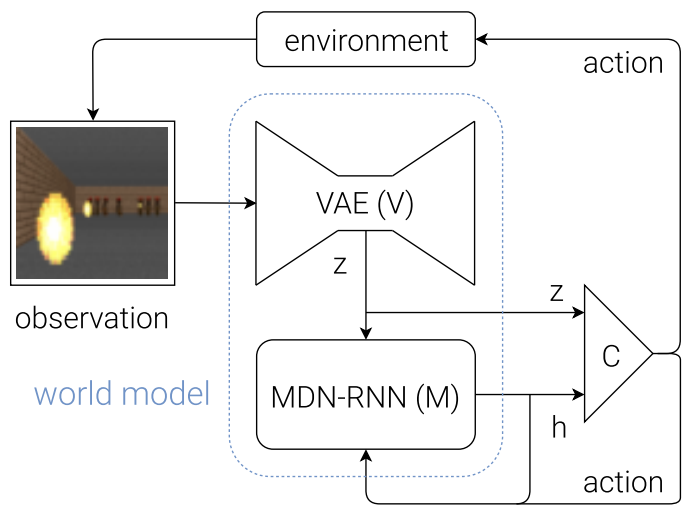
\includegraphics[width=0.5\textwidth]{images/world_model_overview.png}
\caption{flow diagram of the Agent model}
\end{figure}

\begin{itemize}
    \item VAE Model: encode the frame into a small latent vector $z_t$;
    \item MDN-RNN: mixture density network combined with a RNN, $P(z_{t+1}|a_t, z_t, h_t)$, predict the next latent vector $z_{t+1}$;
    \item Controller:  single layer linear model, $a_t = W_c [z_t \hspace{0.5em} h_t] + b_c$
\end{itemize}

\section{Survey from Qazi}

Qazi \cite{qazi2025generativeaiworldmodels} categorizes existing research into three medical subdomains and introduces a capability rubric ranging from L1 to L4. The work further identifies four key limitations of clinical reliability.

\subsection{Capability Rubric}

\begin{itemize}
    \item \textbf{L1 - temporal prediction}: If we continue along the current path, what will the future look like?
    \item \textbf{L2 - action-conditioned prediction}: What will the future look like if given action A?
    \item \textbf{L3 - counterfactual rollouts for decision-making}: Should we give A or B? Which is better for the patient, and can we work out what would happen in other possible cases that did not take place.
    \item \textbf{L4 - planning/control}: The model's internal reasoning is truly integrated into the decision-making loop. The planner searches for action sequences, actions are executed, new observations are returned to update the state, and planning proceeds again to form a closed loop. Ultrasound probe navigation can serve as a reference.
\end{itemize}

\noindent Mathematically, L3 performs Monte Carlo appoximation of the g-formula: conditioned on historical observations and the queried action sequence, it samples subsequent states step by step. Two core mechanisms are incorporated: \textbf{support set constraints} and \textbf{uncertainty penalty}. The support set constraint works as a rollout-side safety fuse: during rollout, if the agent enters regions with no patient data or no empirical evidence, it rejects further prediction and halts rollout. The uncertainty penalty imposes penalties for out-of-distribution extrapolation outside the model's training manifold. Without this penalty, the computed expectation tends to be overly optimistic and yields substantial bias. Note this expectation is estimated under model-based reinforcement learning rather than from the real cilinical environment. Consequently, it imposes a "tax" on unknown, ungrounded regions.

\subsection{Quotes}

\begin{itemize}
    \item the growing clinical data underscore the importance of AI-driven solutions to improve the quality and efficiency of care.
    \item world models learn multimodal, temporally coherent, action-conditioned representations, which reflect the physical and casual structure of care.
    \item world models learn predictive dynamics to enable mutistep rollouts, counterfactual evaluation and planning.
    \item generative models lack grounding in the physical, spatial, and casual structure of clinical reality, and can produce plausible but incorrect outputs with dangerous consequences.
    \item predictive dynamics: given $s_t$ and $a_t$, predict $s_{t+1}$, or via future-latent predictive objectives (JEPA), the joint embedding predictive architecture(JEPA), which has been proposed as a unified framework for predictive learning, \textbf{learn presentations by predicting future latent embedding rather than raw observations}.
    \item WMs can integrate multimodal patient data into a unified latent state, simulate how the state evolves under different interventions, and thus enable critical what-if analyses for decision making.
    \item application areas: medical imaging and diagnostics, disease progression modeling, robotic surgery \& surgical planning.
\end{itemize}



\printbibliography

\end{document}